\documentclass[10pt]{article}
\setlength{\topmargin}{-0.5in}
\setlength{\textwidth}{6.5in}
\setlength{\oddsidemargin}{0in}
\setlength{\textheight}{9in}

%\usepackage{multirow}
%\usepackage{rotating}
\usepackage{bm}
\usepackage[fleqn]{amsmath}
\usepackage{stmaryrd}
\usepackage{natbib}
\usepackage{palatino}
\usepackage{url}
\usepackage{graphicx}
\usepackage{mathtools}
\usepackage[group-separator={,}]{siunitx}

\DeclarePairedDelimiter\floor{\lfloor}{\rfloor}

\begin{document}

\title{CSE 417A: Homework 1 Solution Sketch}


\maketitle

\noindent \textbf{Note:} These are not intended to be comprehensive,
just to help you see what the answers should be.

\begin{enumerate}

\item[Problem 1.3]
\begin{itemize}
    \item[(a)] By definition, $\bm{w}^*$ separates the data. Therefore, $y_n(\bm{w}^{*T}\bm{x}_n) > 0$ for every $n$, and so $\rho>0$.
    \item[(b)] We first show $\bm{w}^T(t)\bm{w}^* \geq \bm{w}^T(t-1)\bm{w}^*+\rho$.\\
    Let $\bm{x}(t-1)$, $y(t-1)$ be the misclassified example at $t-1$, 
    from PLA, we have $\bm{w}(t)=\bm{w}(t-1) + y(t-1)\bm{x}(t-1)$.
    Therefore,
    \[
        \bm{w}^T(t)\bm{w}^* = \bm{w}^T(t-1)\bm{w}^* + y(t)\bm{x}^T(t)\bm{w}^* \geq \bm{w}^T(t-1)\bm{w}^* + \rho
    \]
    Next we prove $\bm{w}^T(t)\bm{w}^* \geq t \rho$ by induction\\
    Since $\bm{w}(0) = \bm{0}$. The statement is true at $t=0$.
    Assume $\bm{w}^T(t)\bm{w}^* \geq t \rho$ is true at $t$. Using the above result, we have 
    \[
        \bm{w}^T(t+1)\bm{w}^* \geq \bm{w}^T(t)\bm{w}^* + \rho \geq (t+1)\rho
    \]
    \item[(c)] Again, we have $\bm{w}(t)=\bm{w}(t-1) + y(t-1)\bm{x}(t-1)$, so
    \[
        \|\bm{w}(t)\|^2 = \|\bm{w}(t-1)\|+\|\bm{x}(t-1)\|^2 + 2y(t-1)\bm{w}^T(t-1)\bm{x}(t-1)
    \]
    Since $\bm{x}(t-1)$, $y(t-1)$ is the misclassified example at $t-1$, $y_t\bm{w}^T(t-1)\bm{x}_t\leq0$. 
    Therefore $\|\bm{w}(t)\|^2 \leq \|\bm{w}(t-1)\|+\|\bm{x}(t-1)\|^2$.
    \item[(d)] 
    We prove by induction.
    Since $\bm{w}(0) = \bm{0}$. The statement is true at $t=0$.
    Assume the statement is true at $t-1$, i.e., $\|\bm{w}(t-1)\|^2 \leq (t-1)R^2$. 
    Since $\bm{w}(t)=\bm{w}(t-1) + y(t-1)\bm{x}(t-1)$,
    we have 
    \[
        \|\bm{w}(t)\|^2 \leq \|\bm{w}(t-1)\|^2 + \|\bm{x}(t-1)\|^2 \leq \|\bm{w}(t-1)\|^2 + R^2 \leq (t-1)R^2  + R^2 \leq tR^2
    \]
    \item[(e)] Since $\|\bm{w}(t)\|\|\bm{w}^*\| \geq \bm{w}^T(t)\bm{w}^*$. 
    From (b), we know $\|\bm{w}(t)\|\|\bm{w}^*\| \geq t\rho$.
    From (d), we know $\|\bm{w}(t)\| \leq R\sqrt{t}$. Therefore,
    \[
        R\sqrt{t} \|\bm{w}^*\| \geq \|\bm{w}(t)\|\|\bm{w}^*\|\geq t\rho
    \]
\end{itemize}

\newpage

\item[PLA Expt] An example histogram of the number of iterations
is shown below, without representing four cases that took more than
1000 iterations (the maximum was 3834). If we compare with the bound
derived in class, we see that the bound is \textbf{very} loose, in
fact, orders of magnitude so (see histogram of the log differences
below). 
%For the extra credit, the algorithm is slower to converge when
%the separation between the two classes is smaller (students have to show
%evidence of this to get credit).
\begin{figure}[h]
\begin{center}
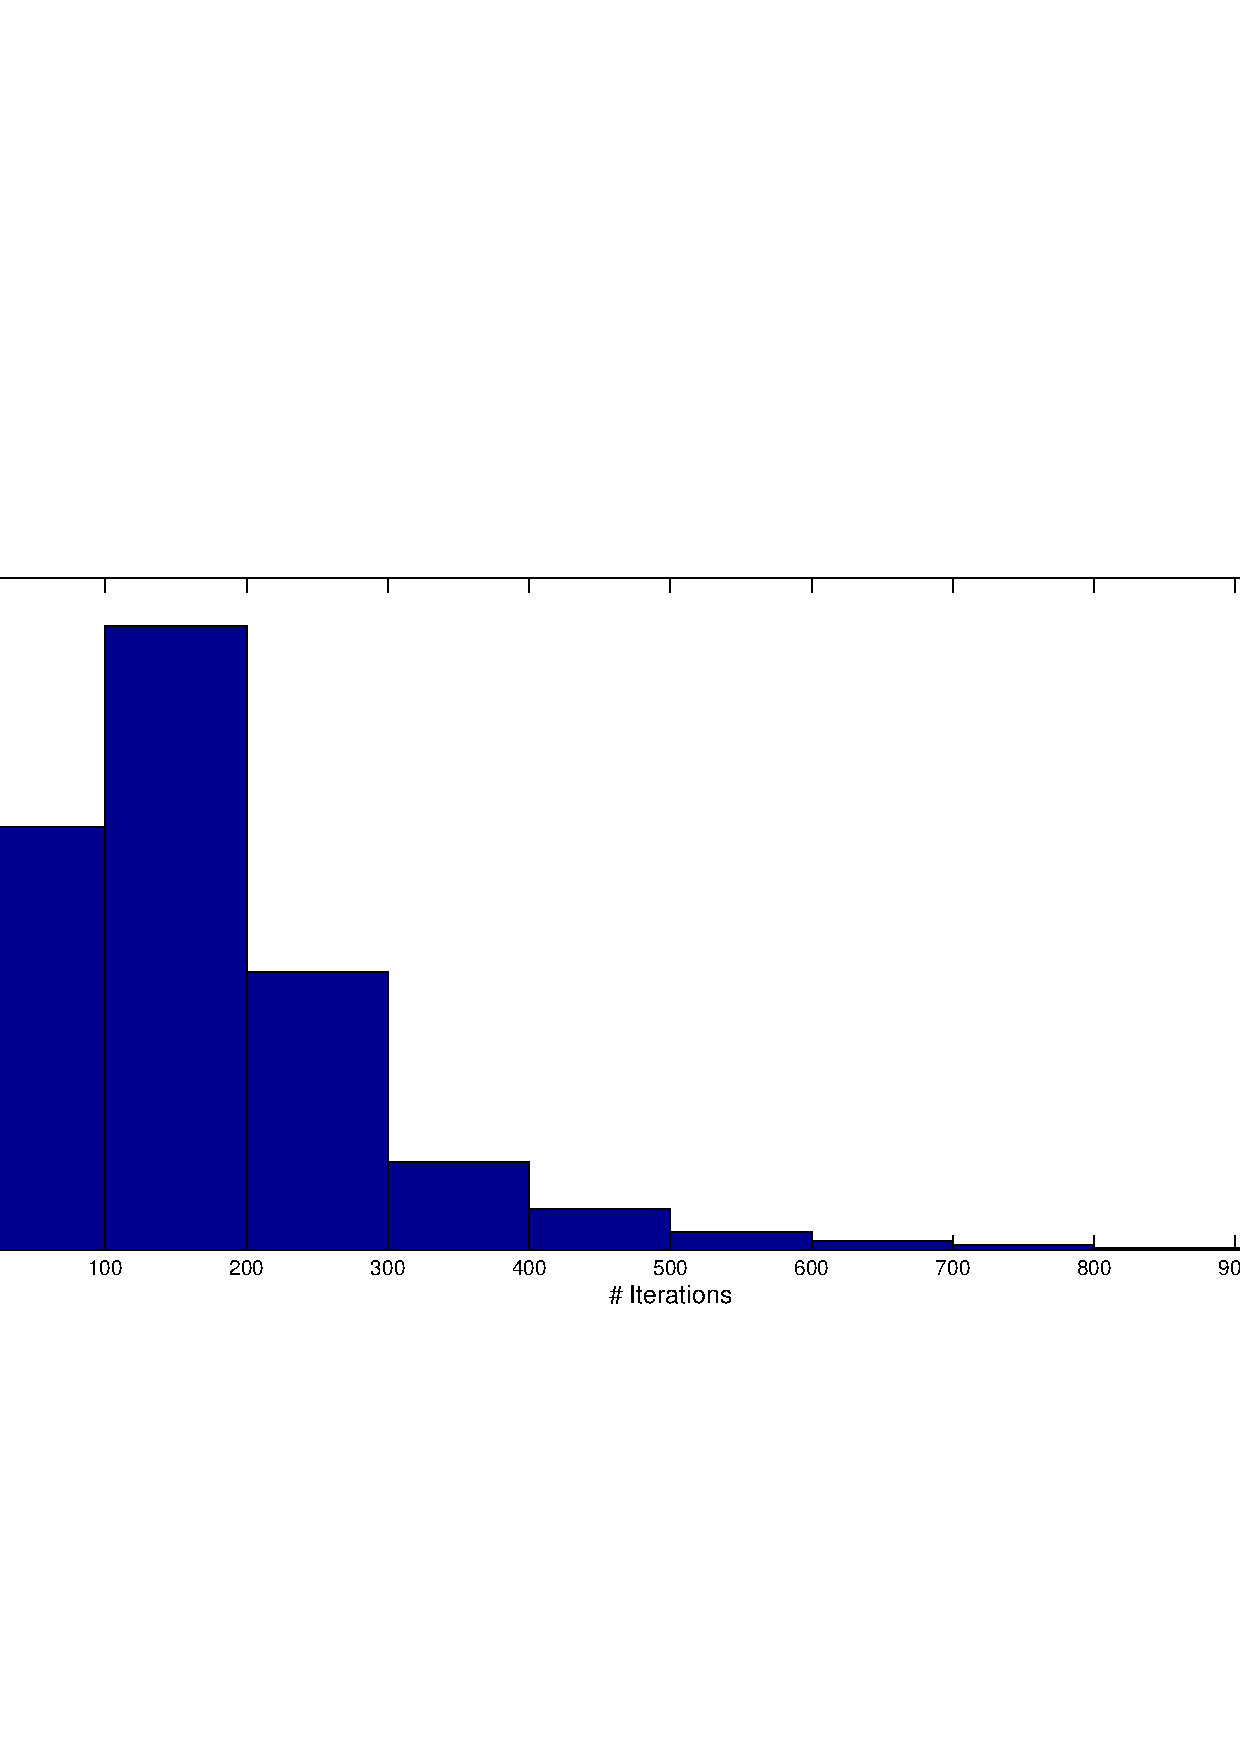
\includegraphics[width=0.45\textwidth]{perceptron_hist}
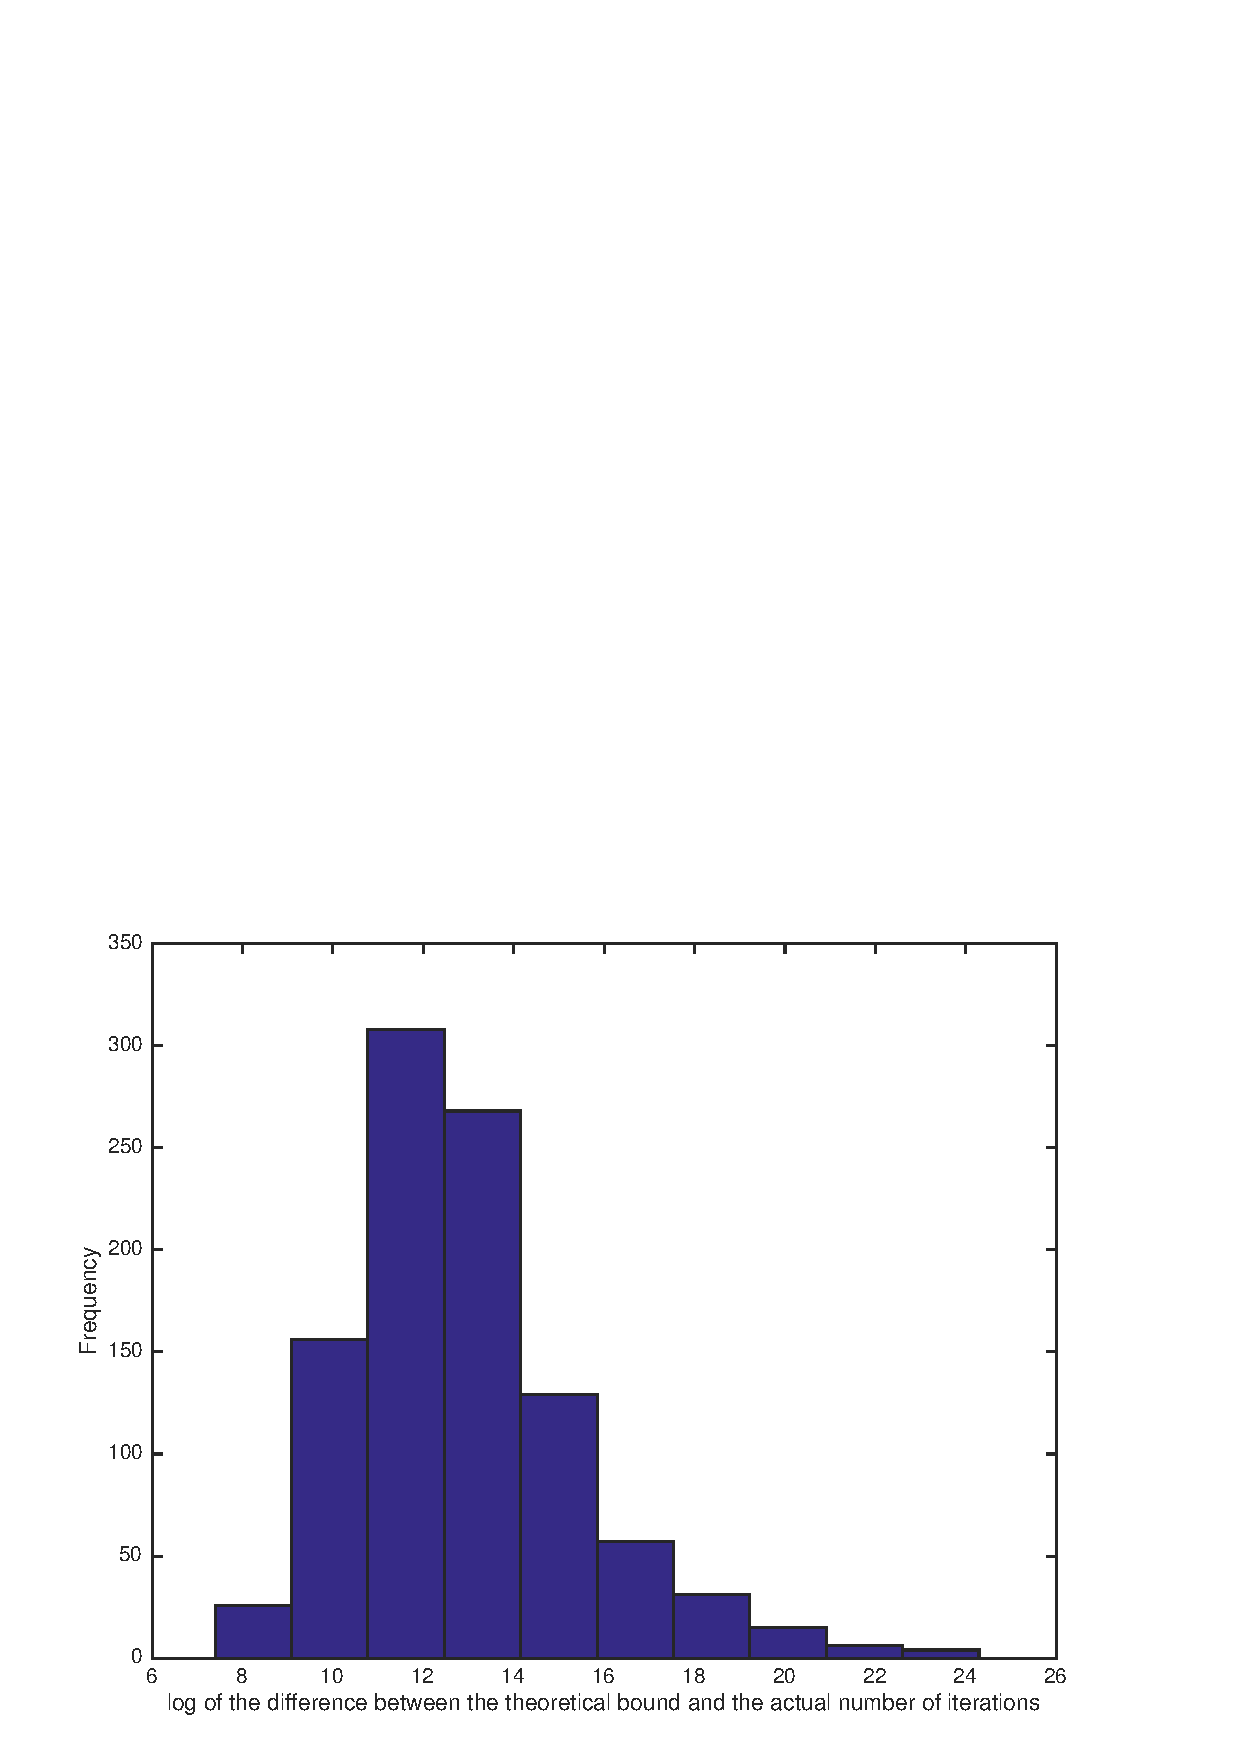
\includegraphics[width=0.45\textwidth]{log_hist}
\end{center}
\end{figure}
  

\item[Exercise 1.10] For part (a), $\mu = 0.5$ for all the coins. A
single line of matlab code that works is 
\begin{verbatim}
mean(randi([0,1],10,1000),1)
\end{verbatim}

For parts (b) and (c), your graphs should look something like this
(the histograms for the random coin and coin 1 should look almost
identical, so we only show one of them here):

\begin{figure}[h]
\begin{center}
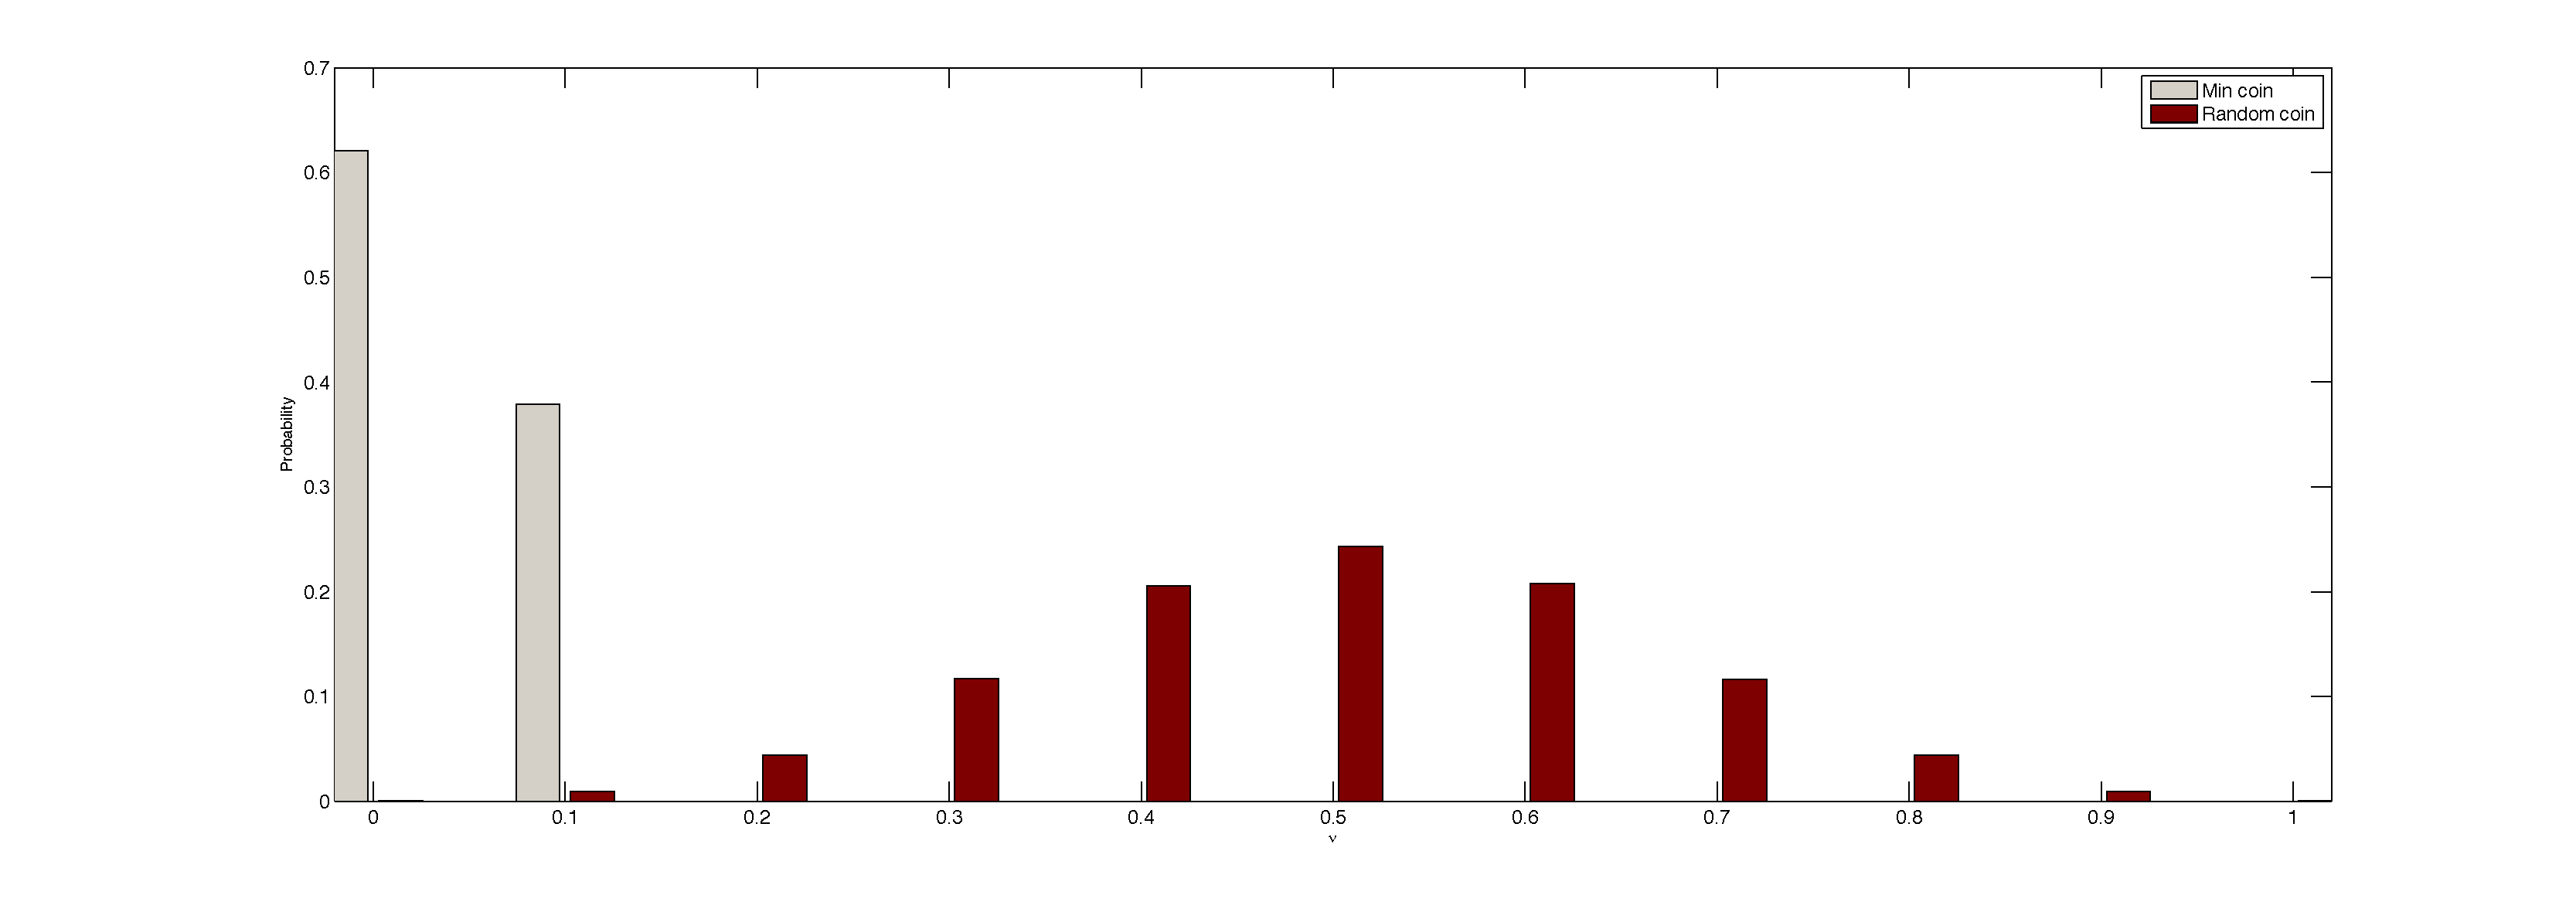
\includegraphics[width=0.8\textwidth]{coin_hist}
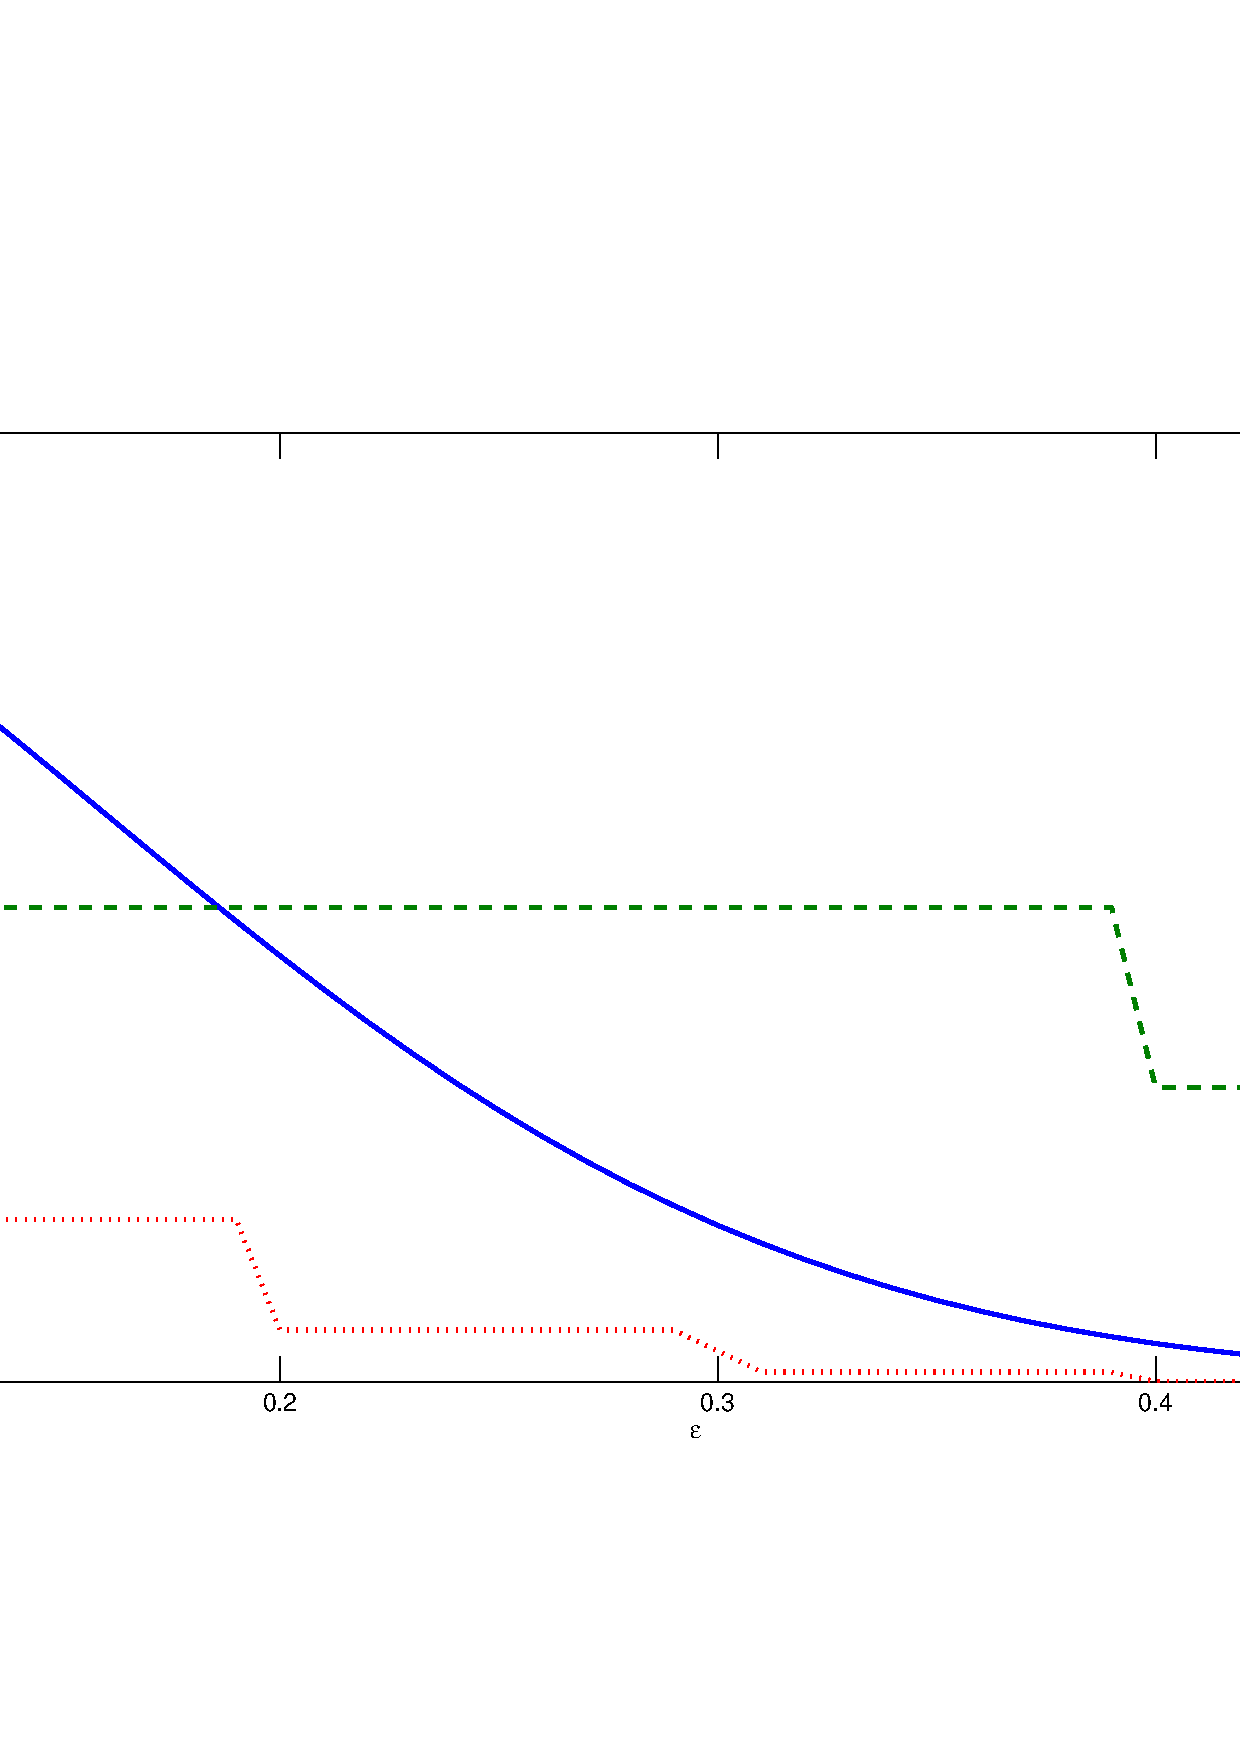
\includegraphics[width=0.8\textwidth]{coin_bounds}
 \end{center}
\end{figure}


For parts (d) and (e), the main thing is that coin 1 and the random
coin are both the equivalent of hypotheses that are selected before
looking at the data, so the Hoeffding bound applies (it's hypothesis
verification). On the other hand the data is used to choose the
``minimum'' coin out of many, so the bound doesn't apply, equivalent
to the multiple (1000) bins model in the text that we discussed in
class. 


\item[Problem 1.8] For part (a) note that $E(t) = E(t | t < \alpha) \Pr (t <
  \alpha) + E(t | t \geq \alpha) \Pr (t \geq \alpha)$. 
  Since the first term is non-negative and $E(t | t \geq
  \alpha) \geq \alpha$, we have 
  \[ E(t) \leq \alpha\Pr(t\geq \alpha).\]

  For part (b), let $t = (u - \mu)^2$, which is non-negative. Now,
  $E(t) = \sigma^2$. Apply part (a) to $t$:
  \[ \Pr ((u - \mu)^2 \geq \alpha) = \Pr (t \geq \alpha) \leq
  \frac{E(t)}{\alpha} = \frac{\sigma^2}{\alpha} \]

For part (c), since $u$ is the sum of $N$ i.i.d. $u_n$, each with
variance $\sigma^2$, the variance of $u$ is $\sigma^2 / N$ (standard
result). Now, applying part (b) with the variance $\sigma^2/N$ gives
us the result.

\item[Problem 1.12] Part (a) is a standard, simple minimization.
  $\frac{\partial E_{\text{in}} (h)}{\partial h} = \sum_{n=1}^{N} (2h -
2y_n)$. Setting to zero, we get $h = \frac{\sum_{n=1}^{N} y_n}{N}$ and
since the second derivative is positive, this is a minimum. 
  
Part (b) can be done in a couple of different ways: one is to split it
up piecewise for minimization. Alternatively, here's a nice proof. 
If you choose any point that is not a median, you must have more points
either on the left or on the right of that point. Assume you have more
points on the left, that is $\sum_{n} \llbracket y_n \geq h
\rrbracket < \sum_{n} \llbracket y_n \leq h \rrbracket$. Then, if
you decrease $h$ by $\delta$ without changing how many points are on
each side, you decrease the error by $\delta (\sum_{n} \llbracket y_n
\leq h \rrbracket - \sum_{n} \llbracket y_n \geq h \rrbracket) > 0$. A
similar argument applies if you have more points on the
right. Therefore, $E_{\text{in}}$ can only be minimized if $\sum_{n} \llbracket y_n \geq h
\rrbracket = \sum_{n} \llbracket y_n \leq h \rrbracket$. 

  Finally, for part (c), $h_{\text{mean}} \rightarrow \infty$ but
  $h_{\text{med}}$ is not affected.


\item[Problem 2.3]
  \begin{itemize}
    \item[(a)] First count dichotomies that have at least one positive
      and one negative point. There are $N-1$ intervals between $N$
      points where one can start a positive or negative ray, so there
      are $2(N-1)$ such dichotomies. There are two more that are all
      positive and all negative, giving a total of $2N$, thus
      $d_{\text{VC}} = 2$ (3 is a break point, 2 is not).

    \item[(b)] Positive or negative intervals alone can implement $1 +
      \binom{N+1}{2}$. Just using $2(1 + \binom{N+1}{2})$ overcounts
      those dichotomies that can be implemented by both -- that number
      is in fact exactly equal to the number that can be implemented
      by the positive or negative ray, so the total number that can be
      implemented is $2(1 + \binom{N+1}{2}) - 2N = N^2 - N +2$. $k=3$
      is not a break point, but $k=4$ is, so $d_{\text{VC}} = 3$. 

    \item[(c)] In terms of dichotomies, this is equivalent to positive
      intervals on the positive real numbers (think about it as
      choosing the radius). So this is again $1 + \binom{N+1}{2}$.
      $d_{\text{VC}} = 2$. 

%  \item[Problem 2.8] $2^{\floor*{\sqrt{N}}}$ and $2^{\floor*{N/2}}$ cannot be
%    growth functions, since they have break points but are not
%    polynomial in $N$. More subtly, $1 + N + \binom{N}{3}$ doesn't
%    work either, because it has a break point at $k=2$ but is not
%    bounded by a polynomial in $N$ of degree $k-1$, which violates
%    Theorem 2.4. The others are all fine.
     \end{itemize} 

\end{enumerate}


\end{document}
